\documentclass[utf8]{ctexart}


\usepackage{amssymb}
\usepackage{enumerate}
\usepackage[numbers]{natbib} 
\usepackage{geometry}
\geometry{left=3.0cm,right=3.0cm,top=2.5cm,bottom=2.5cm}
\usepackage{fancyhdr}
\pagestyle{fancy}
\setlength{\headheight}{10mm}
\rhead{}
\lhead{}
\fancyhead[C]{
	\begingroup
	\setlength{\tabcolsep}{10pt} % Default value: 6pt
	\renewcommand{\arraystretch}{1.5} % Default value: 1
	\begin{tabular}{ccc}
		& \large{\textbf{液晶电光效应综合实验报告}} &  \\
		少年班学院 \qquad \qquad & 刘子安 PB20000069 & \qquad \today
	\end{tabular}
	\endgroup
}   %在此处插入作者信息,改变页眉,此页眉是由我设计的,类似于实验报告纸
\fancyfoot[C]{ 第 {\thepage} 页,共 \pageref{unknown} 页}
\renewcommand{\headrulewidth}{0pt}

\usepackage{multirow} % 单元格合并

\usepackage{graphicx}

\usepackage{siunitx} % 单位

\begin{document}
	
	\subsection*{1.实验目的}	
	\begin{itemize}
		\item  根据液晶的电光效应特性,可制成光开关器件。在掌握液晶光开关的基本工作原理的基础上,测量
		液晶光开关的电光特性曲线,并由电光特性曲线得到液晶的阈值电压和关断电压。
		\item  测量驱动电压周期变化时,液晶光开关的时间响应曲线,并由时间响应曲线得到液晶的上升时间和
		下降时间。
		\item  测量由液晶光开关矩阵所构成的液晶显示器的视角特性以及在不同视角下的对比度,了解液晶光开
		关的工作条件。
	\end{itemize}
	\subsection*{2.实验器材} 
	液晶光开关电光特性综合实验仪,包括发射器,液晶版,接收器,以及各种按钮和电压及透过率显示屏。
	\subsection*{3.实验原理}
	\subsubsection*{液晶光开关工作原理}
	对于常用的TN(扭曲向列)型液晶,其结构如图一所示:
	\begin{figure}[htbp]
		\centering
		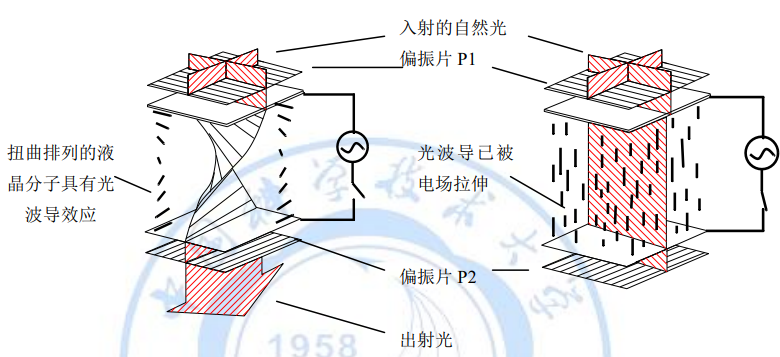
\includegraphics[scale=0.8]{1.png}
		\caption{液晶光开关的工作原理}
	\end{figure}
	在未加驱动电压的情况下,来自光源的自然光经过偏振片 P1 后只剩下平行于透光轴的线偏振光,
	该线偏振光到达输出面时,其偏振面旋转了 90°,如图 1 左图所示。这时光的偏振面与 P2 的透光轴平
	行,因而有光通过。

	在施加足够电压情况下(一般为 1~2 伏),在静电场的作用下,除了基片附近的液晶分子被基片“锚
	定”以外,其他液晶分子趋于平行于电场方向排列(上下两电极形成的空间相当于平行板电容器)。于
	是原来的扭曲结构被破坏,成了均匀结构,如图 1 右图所示。从 P1 透射出来的偏振光的偏振方向在液
	晶中传播时不再旋转,保持原来的偏振方向到达下电极。这时光的偏振方向与 P2 正交,因而光被关断。
	\subsubsection*{液晶光开关电光特性}
	当光线垂直液晶面入射时,液晶相对透过率随着外部所加的电压不同而不同,如图2所示。并且
	可以从相对透过率-电压曲线中得到其阈值电压(透过率为$90\%$时的电压)
	和关断电压(透过率为$10\%$的电压)。
	\begin{figure}[htbp]
		\centering
		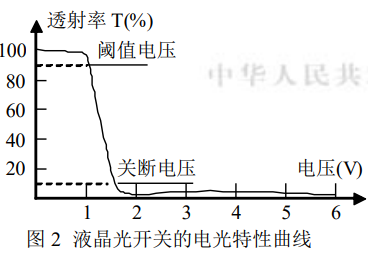
\includegraphics[scale=0.7]{2.png}
		\caption{液晶光开关的电光特性曲线}
	\end{figure}

	\subsubsection*{液晶光开关的时间响应特性}
	加上(或去掉)驱动电压会使液晶的开关状态发生改变,这个状态的改变需要一定时间,反映在
	时间响应曲线上,使用上升时间$\tau_r$(透过率从$10\%$升到$90\%$)和
	下降时间$\tau_d$(透过率从$90\%$降到$10\%$)描述。

	\subsubsection*{液晶光开关的视角特性}
	液晶光开关的视角特性表示为对比度与视角的关系。对比度定义为光开关打开和关断时
	透射光强度比。一般认为对比度大于5时可以得到满意的图像,小于2时图像就模糊不清了。

	通过理论计算可以得到,液晶的对比度与垂直视角,水平视角都有关,并且具有非对称性。

	
	\subsection*{4.数据分析及处理}
	\subsubsection*{(1)数据记录及处理}
	\textbf{1.液晶光开关电光特性测量}

	\begin{table}[htbp]
		\caption{液晶光开关电光特性测量}
		\label{table1}
		\centering
		\scalebox{0.77}{
			\begin{tabular}{|c|c|c|c|c|c|c|c|c|c|c|c|c|c|c|c|c|c|}
				\hline
				\multicolumn{2}{|c|}{电压(伏)} & 0 & 0.5 & 0.8 & 1.0 & 1.1 & 1.2 & 1.3 & 1.4 & 1.5 & 1.6 & 1.7 & 2.0 & 3.0 & 4.0 & 5.0 & 6.0 \\
				\hline
				\multicolumn{1}{|c|}{\multirow{4}{*}{}透} &  1  & 100 & 96.8 & 80.7 & 46.9 & 30.9 & 19.3 & 11.7 & 7.6 & 5.3 & 4.2 & 3.8 & 4.0 & 4.3 & 3.8 & 4.5 & 3.2 \\
				\cline{2-18}
				\multicolumn{1}{|c|}{射} & 2 & 91.0 & 90.7 & 75.3 & 43.2 & 29.0 & 18.5 & 11.4 & 7.4 & 5.1 & 4.1 & 3.8 & 4.0 & 4.3 & 3.8 & 3.5 & 3.2 \\
				\cline{2-18}
				\multicolumn{1}{|c|}{率} & 3 & 91.0 & 90.6 & 75.7 & 43.3 & 29.4 & 18.4 & 11.5 & 7.4 & 5.1 & 4.0 & 3.7 & 4.0 & 4.2 & 3.7 & 3.4 & 3.1 \\
				\cline{2-18}
				\multicolumn{1}{|c|}{(\%)} & 平均 & 91.0 & 90.65 & 75.5 & 43.25 & 29.2 & 18.45 & 11.45 & 7.4 & 5.1 & 4.05 & 3.75 & 4.0 & 4.25 & 3.75 & 3.45 & 3.15 \\
				\hline
	
			\end{tabular}
		}
	\end{table}
	所得的数据如表\ref{table1}所示,从表中我们可以发现第一次的数据与第二、三次相差较大,这可能是由于在第一次测量之后环境的改变造成的,角度的移动或者光环境的改变都会
	造成所得透过率的变化,于是我们舍去第一组数据,使用第二组和第三组数据计算平均值并绘制电光特性曲线。
	\begin{figure}[htbp]
		\centering
		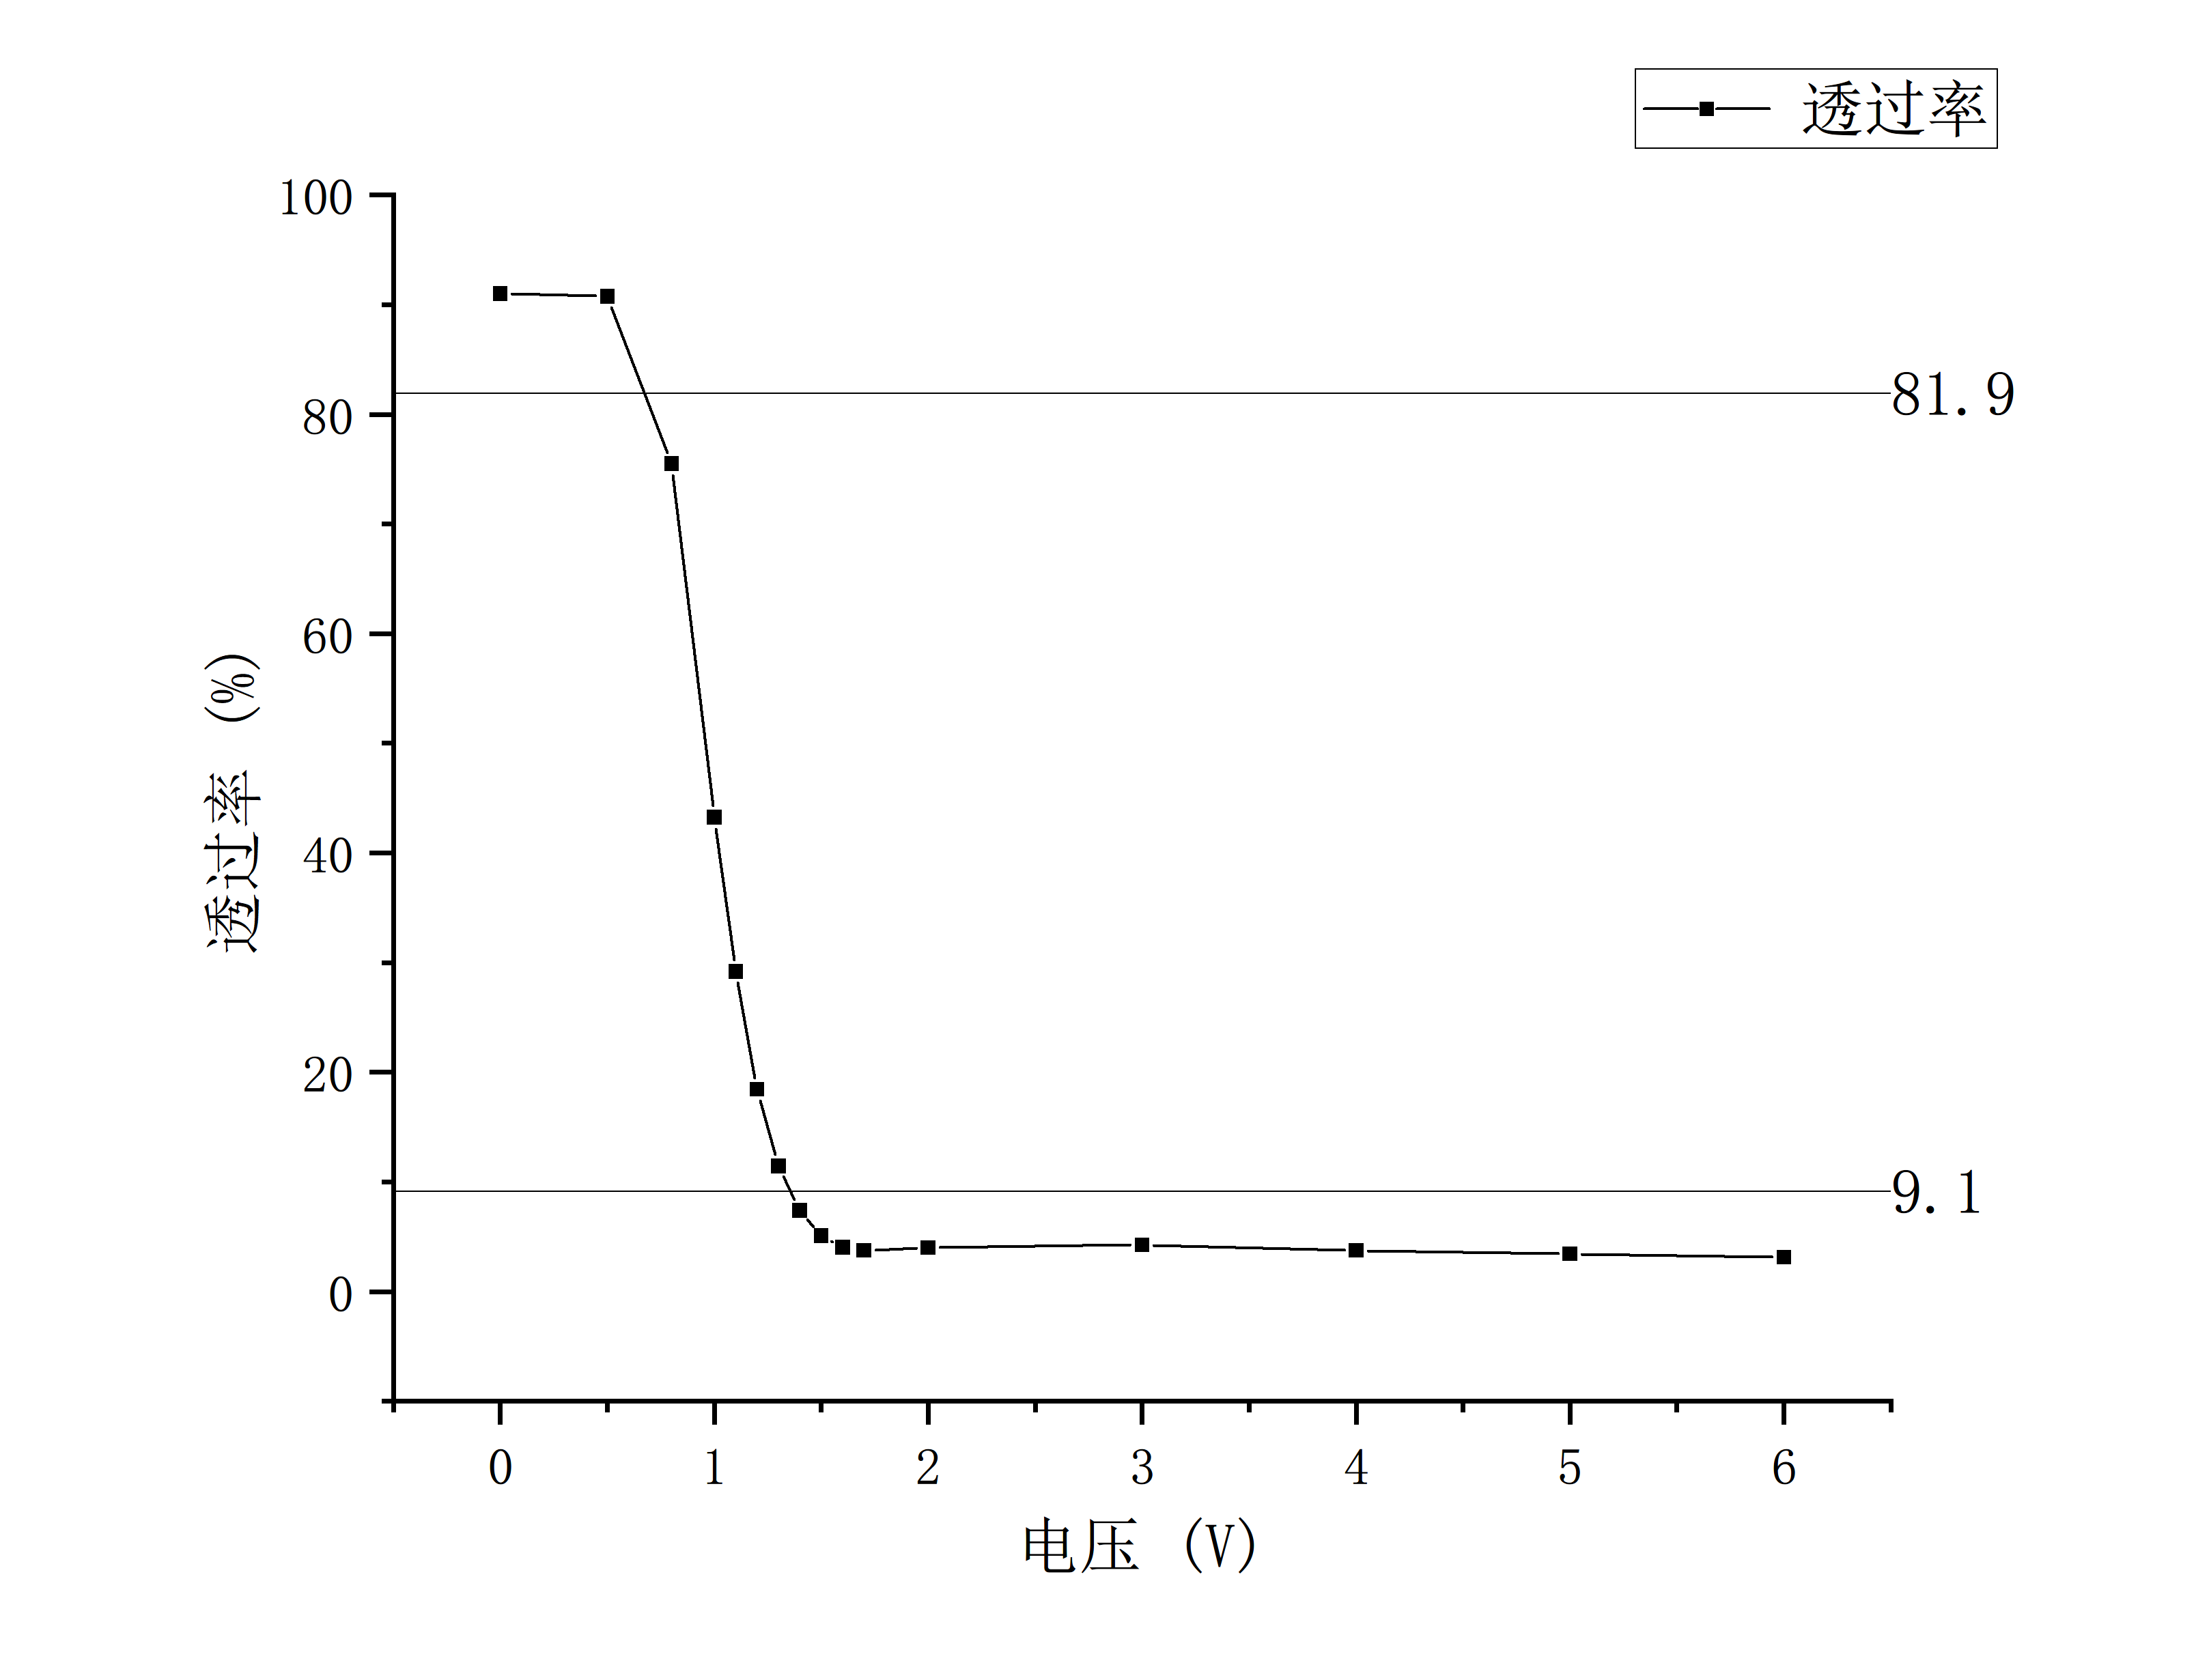
\includegraphics[scale=0.45]{3.png}
		\caption{液晶电光特性曲线}
	\end{figure}

	在图中绘制出透过率-电压的关系曲线以及透过率为$91\% \times 0.9 = 81.9\%$和$91\% \times 0.1 = 9.1\%$的直线,
	可以得到两个交点对应的阈值电压$V_1$和关断电压$V_2$分别为:
	$$
		V_1 = \qty{0.68}{V}
	$$
	$$
		V_2 = \qty{1.35}{V}
	$$
	
	\textbf{2. 液晶时间响应的测量}

	使用示波器可以直接测得液晶的响应时间为:
	\begin{table}[htbp]
		\caption{响应时间}
		\label{table2}
		\centering
		\begin{tabular}{|c|c|c|c|c|}
			\hline
			次数 & 1 & 2 & 3 & 平均 \\
			\hline
			上升时间$\tau_r(\unit{ms})$ & 34.00 & 38.00 & 39.00 & 37.00 \\
			\hline
			下降时间$\tau_d(\unit{ms})$ & 19.00 & 21.60 & 19.00 & 19.53 \\
			\hline 
		\end{tabular}
	\end{table}

	于是可知液晶的响应时间为:
	$$\tau_{Total} = \tau_r + \tau_d = 37.00 + 19.53 \unit{ms} = \qty{56.53}{ms}$$

	可得该液晶每秒可达到$1/\tau_{Total} = 17.6 $帧,小于25帧,无法充当电视显示器的液晶材料。响应时间
	应该至多是:
	$$
		\tau = \frac{1}{25} \unit{s} = \qty{40.00}{ms}
	$$

	\textbf{3.液晶光开关视角特性的测量}
	\par
	测得水平方向不同角度的对比度为如表3所示。
	\par
	\begin{table}[htbp]
		\caption{水平方向视角特性}
		\centering
		\scalebox{0.8}{
			\begin{tabular}{|c|c|c|c|c|c|c|c|c|c|c|c|c|c|c|c|c|c|c|}
				\hline
				正角度$^\circ$ & 0 & 5 & 10 & 15 & 20 & 25 & 30 & 35 & 40 & 45 & 50 & 55 & 60 & 65 & 70 & 75 \\
				\hline
				$T_{max}(\qty{0}{V})$ & 100 & 99.7 & 99.5 & 99.3 & 98.9 & 97.8 & 96.0 & 93.7 & 92.0 & 87.2 & 84.2 & 77.3 & 69.1 & 57.7 & 43.4 & 29.4 \\
				\hline
				$T_{min}(\qty{2}{V})$ & 4.1 & 3.9 & 3.7 & 3.4 & 3.2 & 3.2 & 3.3 & 3.5 & 3.6 & 3.5 & 3.4 & 3.4 & 3.4 & 3.2 & 2.6 & 1.9 \\
				\hline
				$T_{max}/T_{min}$ & 24.4 & 25.6 & 26.9 & 29.2 & 30.9 & 30.6 & 29.1 & 26.8 & 25.6 & 24.9 & 24.8 & 22.7 & 20.3 & 18.0 & 16.7 & 15.5 \\
				\hline
				负角度$^\circ$ & 0 & 5 & 10 & 15 & 20 & 25 & 30 & 35 & 40 & 45 & 50 & 55 & 60 & 65 & 70 & 75 \\
				\hline
				$T_{max}(\qty{0}{V})$ & 100 & 100 & 101 & 101 & 102 & 101 & 100 & 98.5 & 97.6 & 93.8 & 90.9 & 84.7 & 77.9 & 69.1 & 56.9 & 40.9 \\
				\hline
				$T_{min}(\qty{2}{V})$ & 4.1 & 4.1 & 4.0 & 3.8 & 3.7 & 3.5 & 3.3 & 3.3 & 3.4 & 3.5 & 3.7 & 3.8 & 3.9 & 3.9 & 3.6 & 2.8 \\
				\hline
				$T_{max}/T_{min}$ & 24.4 & 24.4 & 25.3 & 26.6 & 27.6 & 28.9 & 30.3 & 29.8 & 28.7 & 26.9 & 24.6 & 22.3 & 20.0 & 17.8 & 15.8 & 14.6 \\
				\hline
			\end{tabular}
		}
	\end{table}

	根据表格数据绘制水平方向对比度随入射角变化的曲线:
	\begin{figure}[htbp]
		\centering
		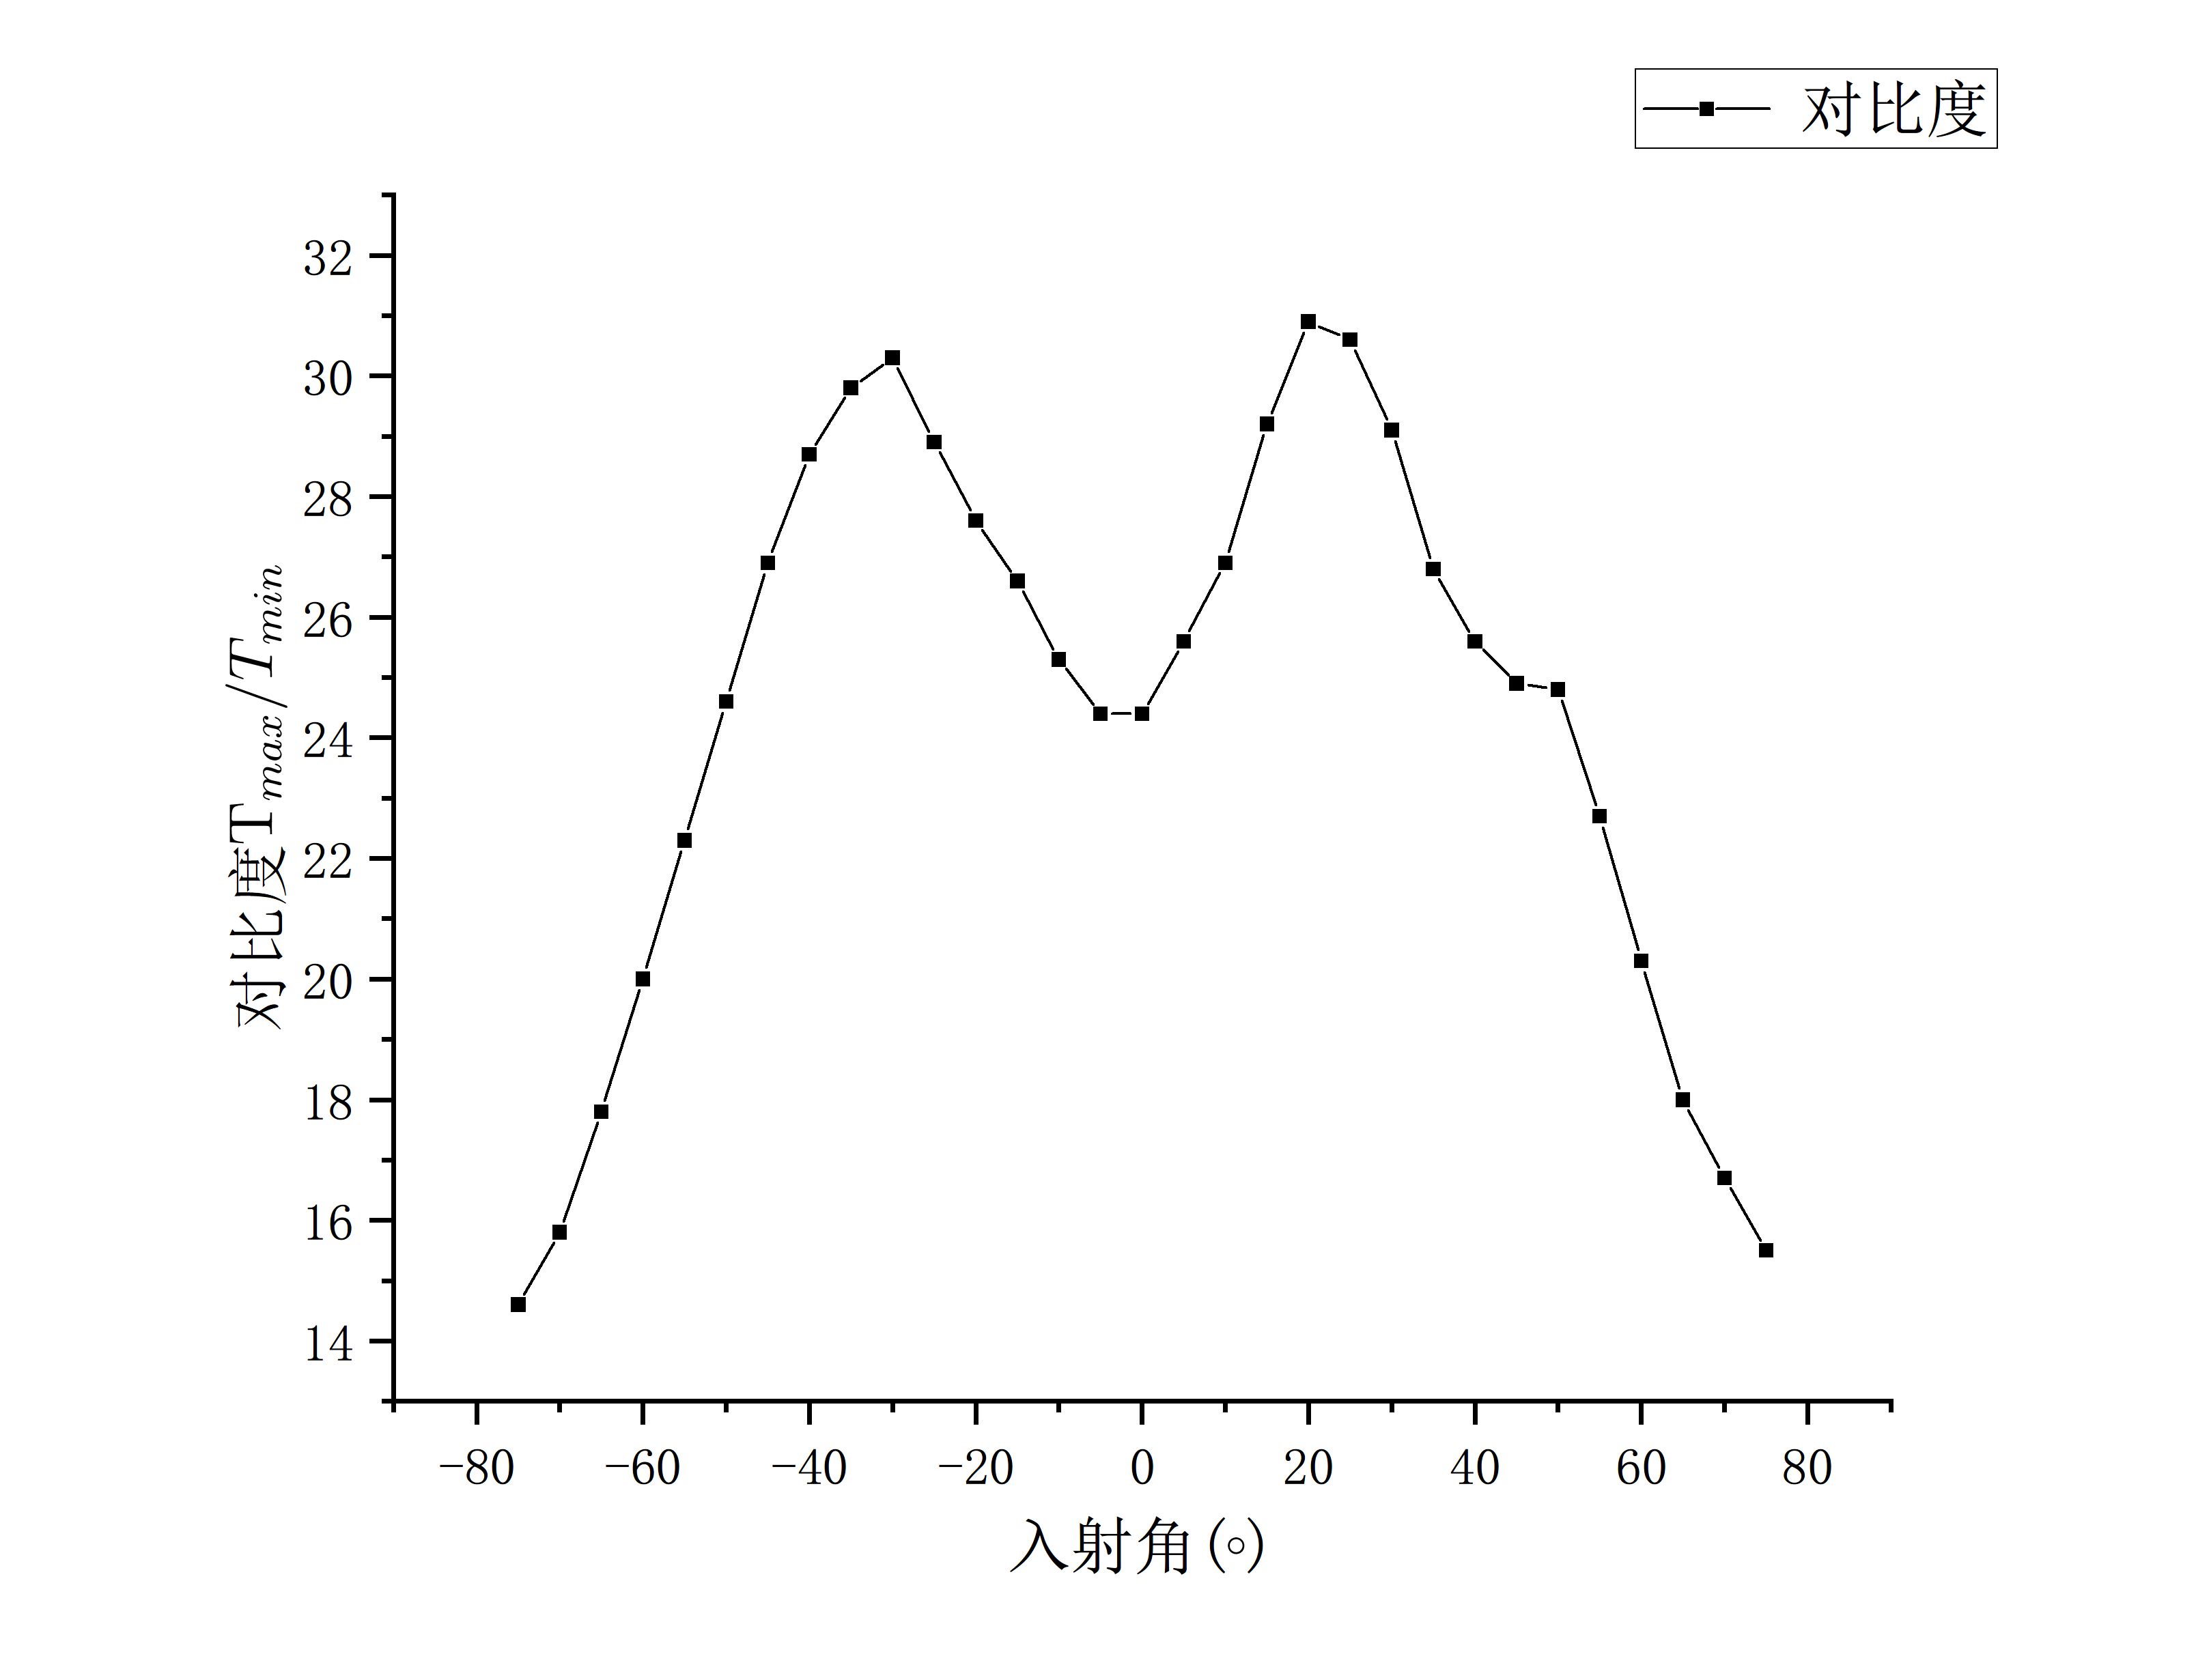
\includegraphics[scale=0.45]{5.png}
		\caption{水平方向对比度随入射角的变化曲线}
	\end{figure}

	将液晶版旋转90度后测得垂直方向上不同角度的对比度为:

	\begin{table}[!htbp]
		\caption{垂直方向视角特性}
		\centering
		\scalebox{0.8}{
			\begin{tabular}{|c|c|c|c|c|c|c|c|c|c|c|c|c|c|c|c|c|c|}
				\hline
				正角度$^\circ$ & 0 & 5 & 10 & 15 & 20 & 25 & 30 & 35 & 40 & 45 & 50 & 55 & 60 & 65 & 70 & 75 \\
				\hline
				$T_{max}(\qty{0}{V})$ & 100 & 99.1 & 97.7 & 95.7 & 92.8 & 89.3 & 86.5 & 83.3 & 79.8 & 76.9 & 74.2 & 71.3 & 68.2 & 61.6 & 50.4 & 36.5 \\
				\hline
				$T_{min}(\qty{2}{V})$ & 3.8 & 5.7 & 8.9 & 14.1 & 20.3 & 27.3 & 35.0 & 42.8 & 49.5 & 55.8 & 59.9 & 62.0 & 62.2 & 58.1 & 48.2 & 36.5 \\
				\hline
				$T_{max}/T_{min}$ & 26.3 & 17.4 & 11.0 & 6.8 & 4.6 & 3.3 & 2.5 & 1.9 & 1.6 & 1.4 & 1.2 & 1.2 & 1.1 & 1.1 & 1.0 & 1.0 \\
				\hline
				负角度$^\circ$ & 0 & 5 & 10 & 15 & 20 & 25 & 30 & 35 & 40 & 45 & 50 & 55 & 60 & 65 & 70 & 75 \\
				\hline
				$T_{max}(\qty{0}{V})$ & 100 & 100 & 100 & 99.4 & 97.8 & 95.6 & 93.6 & 91.4 & 88.0 & 85.8 & 82.4 & 78.4 & 73.6 & 67.3 & 59.7 & 48.0 \\
				\hline
				$T_{min}(\qty{2}{V})$ & 3.8 & 3.5 & 4.4 & 6.8 & 10.6 & 16.0 & 23.0 & 31.8 & 41.2 & 51.4 & 60.3 & 66.0 & 68.2 & 66.1 & 57.1 & 46.9 \\
				\hline
				$T_{max}/T_{min}$ & 26.3 & 28.6 & 22.7 & 14.6 & 9.2 & 6.0 & 4.1 & 2.9 & 2.1 & 1.7 & 1.4 & 1.2 & 1.1 & 1.0 & 1.0 & 1.0 \\
				\hline

			\end{tabular}
		}
	\end{table}

	通过表4绘制出垂直方向对比度随入射角变化的曲线:
	\begin{figure}[htbp]
		\centering
		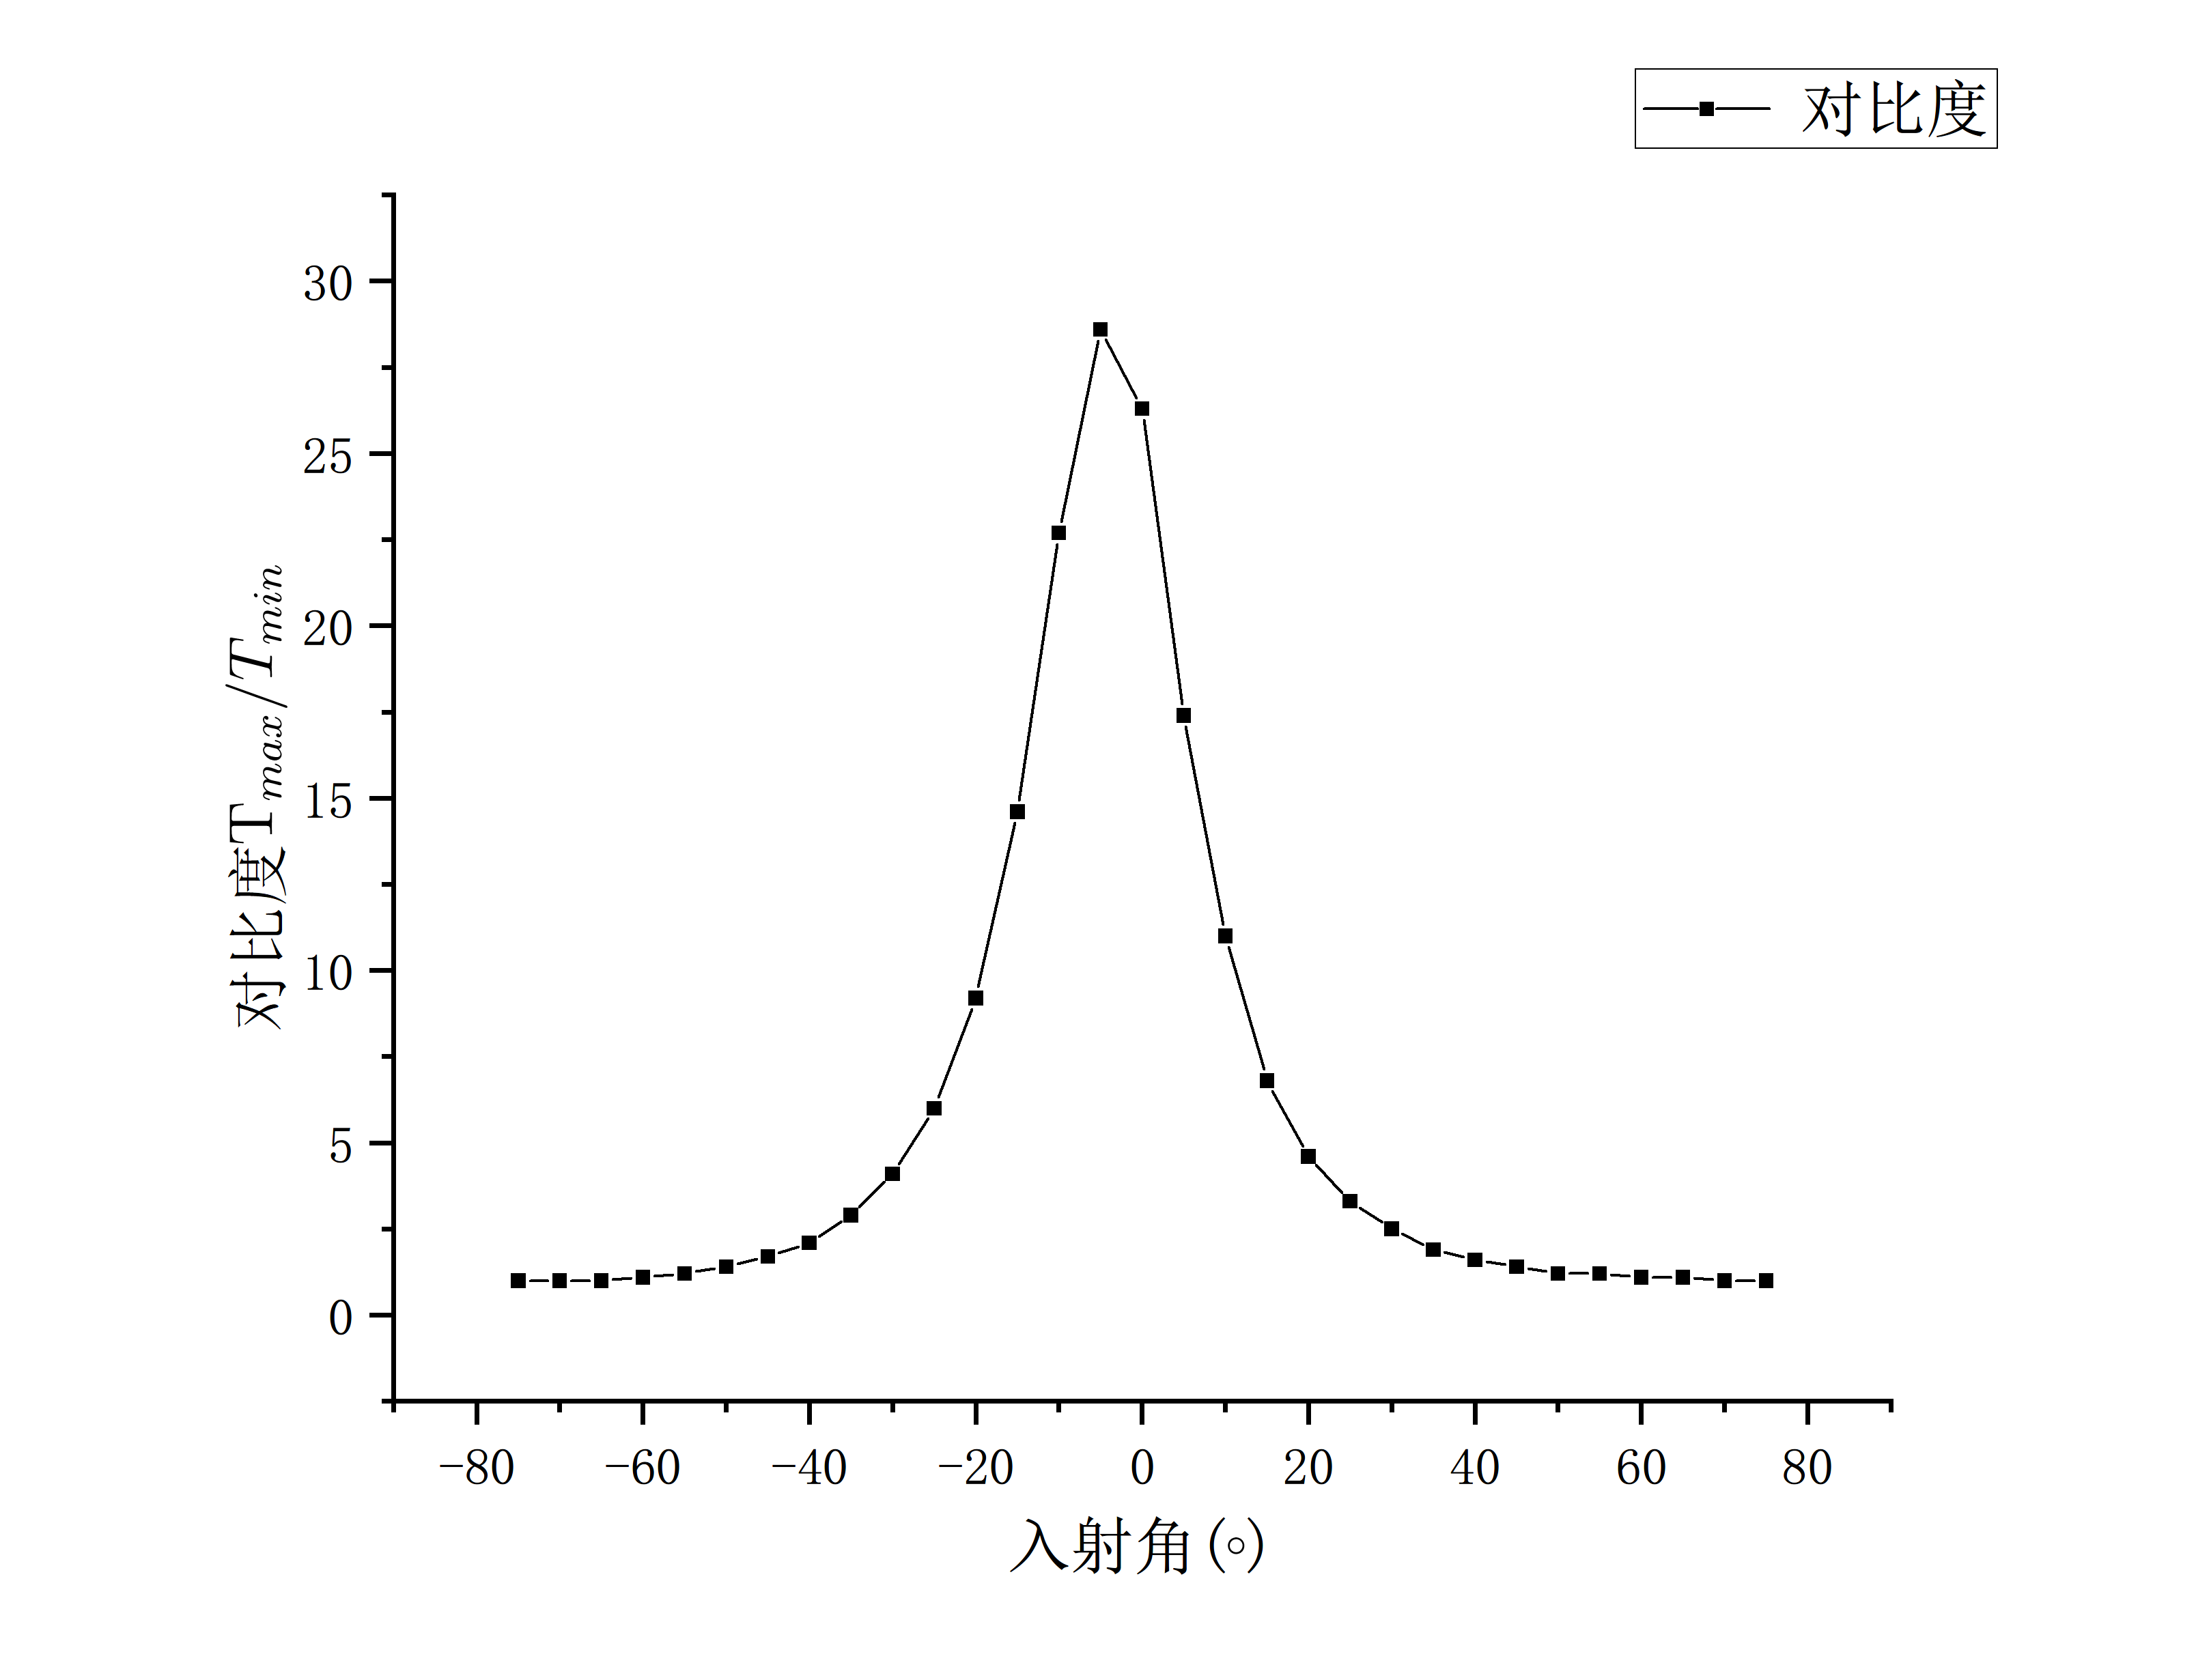
\includegraphics[scale=0.45]{6.png}
		\caption{垂直方向对比度随入射角的变化曲线}
	\end{figure}

	从以上两个表格的数据中我们可以发现,在$-75^\circ$到$75^\circ$之间,水平方向对比度普遍在15以上,
	即水平方向上都显示的比较好。而对于垂直方向,要求对比度大于5,则较好的垂直视角显示范围为$-25^\circ$到$15^\circ$
	之间。

	另外从数据中可以发现,透光率有时候会大于100\%,这是因为该角度的透过率大于$0^\circ$
	时对应的透过率,

	\subsubsection*{(2)误差分析}
	本次实验的主要误差应该来自于仪器的误差,另外在做第一个实验测量液晶光开关
	电光特性时,发现第一次测试校准后,在第二次测试前对桌子有一定磕碰,此后液晶的透过率发生较大改变
	导致第二次与第一次测量相差较大,猜想可能是由于光源的角度不够稳定造成的。
	
	\subsection*{5.思考题}
	\begin{itemize}
		\item [1.] 如何确定本实验所使用的液晶样品是常黑型的还是常白型的。
  		\item []答:由于上述光开关在没有电场的情况下让光透过,加上电场的时候透过率下降,光被关断,因此是常白型光开关。
		\item [2.] 在显示领域中,液晶显示屏(TFT-LCD)替代传统的显示器CRT的主要原因是什么?
  		\item []答:我认为液晶显示屏替代CRT的主要原因有以下几点:
		\begin{itemize}
			\item 界面效果好。LCD液晶屏使用纯平面图的玻璃,且更容易在小总面积显示屏上
			完成高像素。
			\item LCD液晶屏使用数显式插口,而不是像CRT一样选用仿真模拟插口,理论上
			这会使颜色和定位更加精准。
			\item LCD液晶屏不需要射线管,尺寸和重量相对CRT都偏小。
			\item LCD液晶屏的功耗相比CRT要小的多。
		\end{itemize}
	\end{itemize}


	\subsection*{6.总结}
	通过这次实验我了解到了TN型液晶光开关的一些原理和性质,如其电光特性、时间响应还有
	视角特性。通过对视角特性的测量发现水平方向比垂直方向有更好的视角特性,与文献\cite{art1}中一致。

	\bibliographystyle{plain}
	\bibliography{example} % 同文件夹下新建所需的example.bib文件
	
	
	\label{unknown}
\end{document}